\chapter{Application}\label{chpt:application}
\glsresetall

This chapter is about the application that was motivated in section~\ref{sec:intro:problem}. First of 
all the concept is specified. After that the acquisition of data as well as the implementation is 
described.

\section{Concept}\label{sec:app:concept}

The following concept is divided into two parts. The first part covers all the workflows for obtaining a 
trained model and the second part describes how such a trained model can be used for inference on 
new data.

\subsection{Training}\label{subsec:app:training}

\begin{figure}
	\centering
	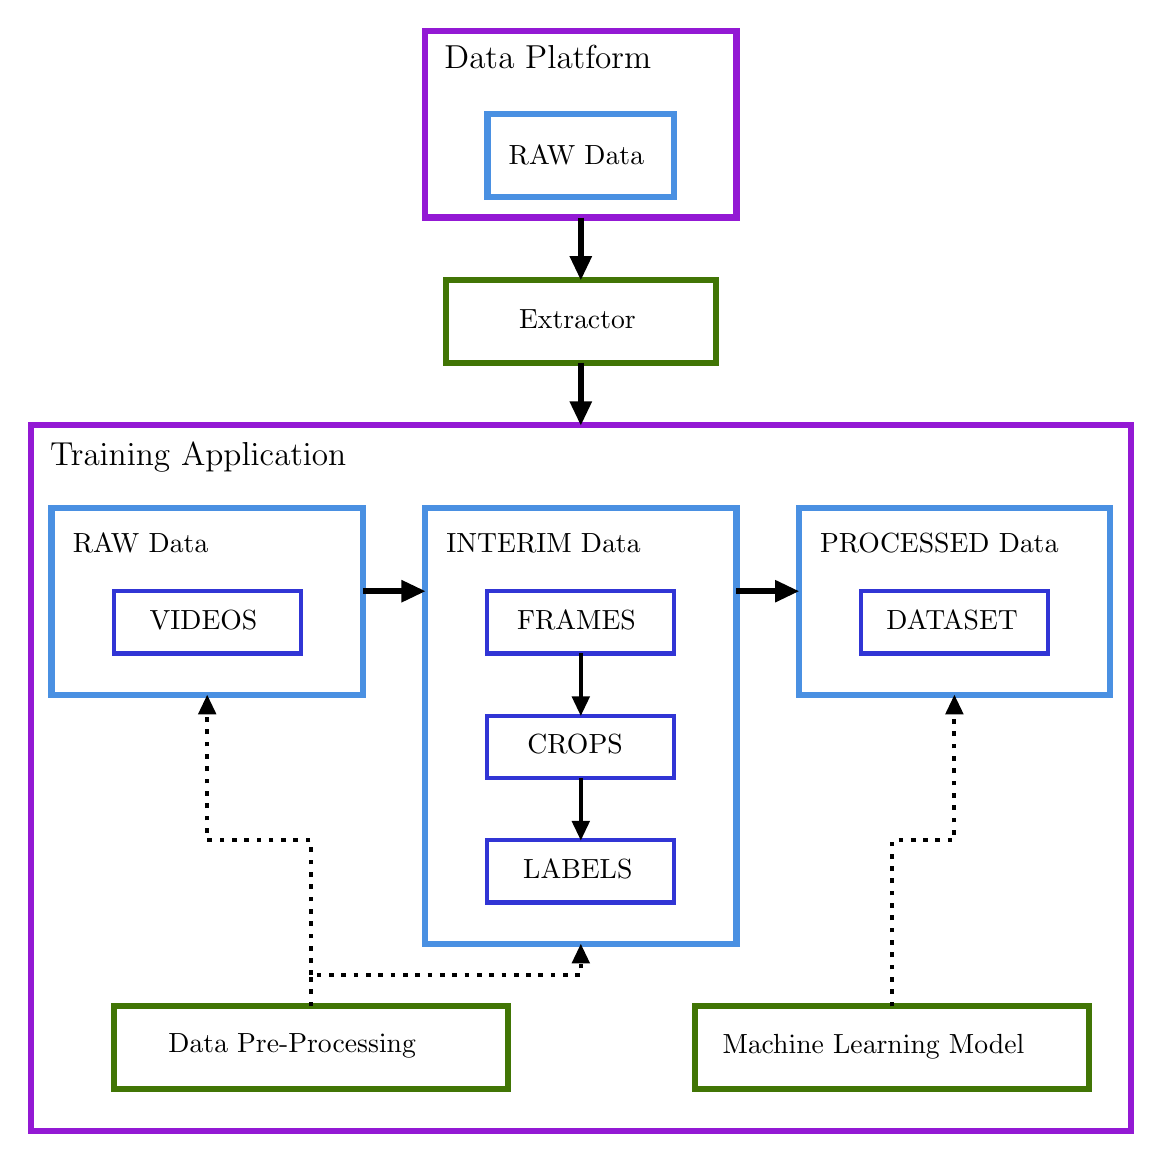
\begin{tikzpicture}[x=0.75pt,y=0.75pt,yscale=-1,xscale=1]
		\draw  [color={rgb, 255:red, 147; green, 25; blue, 212 }  ,draw opacity=1 ][line width=2.25]  
		(250,10) -- (400,10) -- (400,100) -- (250,100) -- cycle ;
		\draw  [color={rgb, 255:red, 147; green, 25; blue, 212 }  ,draw opacity=1 ][line width=2.25]  
		(60,200) -- (590,200) -- (590,540) -- (60,540) -- cycle ;
		\draw  [color={rgb, 255:red, 65; green, 117; blue, 5 }  ,draw opacity=1 ][line width=2.25]  
		(260,130) -- (390,130) -- (390,170) -- (260,170) -- cycle ;
		
		\draw [line width=2.25]    (325,100) -- (325,125) ;
		\draw [shift={(325,130)}, rotate = 270] [fill={rgb, 255:red, 0; green, 0; blue, 0 }  ][line 
		width=0.08]  [draw opacity=0] (11.43,-5.49) -- (0,0) -- (11.43,5.49) -- cycle    ;
		\draw [line width=2.25]    (325,170) -- (325,195) ;
		\draw [shift={(325,200)}, rotate = 270] [fill={rgb, 255:red, 0; green, 0; blue, 0 }  ][line 
		width=0.08]  [draw opacity=0] (11.43,-5.49) -- (0,0) -- (11.43,5.49) -- cycle    ;
		\draw  [color={rgb, 255:red, 74; green, 144; blue, 226 }  ,draw opacity=1 ][line width=2.25]  
		(70,240) -- (220,240) -- (220,330) -- (70,330) -- cycle ;
		\draw  [color={rgb, 255:red, 74; green, 144; blue, 226 }  ,draw opacity=1 ][line width=2.25]  
		(280,50) -- (370,50) -- (370,90) -- (280,90) -- cycle ;
		
		\draw  [color={rgb, 255:red, 65; green, 117; blue, 5 }  ,draw opacity=1 ][line width=2.25]  
		(100,480) -- (290,480) -- (290,520) -- (100,520) -- cycle ;
		
		\draw  [color={rgb, 255:red, 74; green, 144; blue, 226 }  ,draw opacity=1 ][line width=2.25]  
		(250,240) -- (400,240) -- (400,450) -- (250,450) -- cycle ;
		\draw  [color={rgb, 255:red, 49; green, 53; blue, 213 }  ,draw opacity=1 ][line width=1.5]  
		(100,280) -- (190,280) -- (190,310) -- (100,310) -- cycle ;
		\draw  [color={rgb, 255:red, 49; green, 53; blue, 213 }  ,draw opacity=1 ][line width=1.5]  
		(280,280) -- (370,280) -- (370,310) -- (280,310) -- cycle ;
		
		\draw  [color={rgb, 255:red, 49; green, 53; blue, 213 }  ,draw opacity=1 ][line width=1.5]  
		(280,340) -- (370,340) -- (370,370) -- (280,370) -- cycle ;
		
		\draw  [color={rgb, 255:red, 49; green, 53; blue, 213 }  ,draw opacity=1 ][line width=1.5]  
		(280,400) -- (370,400) -- (370,430) -- (280,430) -- cycle ;
		
		\draw [line width=1.5]    (325,310) -- (325,336) ;
		\draw [shift={(325,340)}, rotate = 270] [fill={rgb, 255:red, 0; green, 0; blue, 0 }  ][line 
		width=0.08]  [draw opacity=0] (9.29,-4.46) -- (0,0) -- (9.29,4.46) -- cycle    ;
		\draw [line width=1.5]    (325,370) -- (325,396) ;
		\draw [shift={(325,400)}, rotate = 270] [fill={rgb, 255:red, 0; green, 0; blue, 0 }  ][line 
		width=0.08]  [draw opacity=0] (9.29,-4.46) -- (0,0) -- (9.29,4.46) -- cycle    ;
		\draw [line width=2.25]    (220,280) -- (245,280) ;
		\draw [shift={(250,280)}, rotate = 180] [fill={rgb, 255:red, 0; green, 0; blue, 0 }  ][line 
		width=0.08]  [draw opacity=0] (11.43,-5.49) -- (0,0) -- (11.43,5.49) -- cycle    ;
		\draw  [color={rgb, 255:red, 74; green, 144; blue, 226 }  ,draw opacity=1 ][line width=2.25]  
		(430,240) -- (580,240) -- (580,330) -- (430,330) -- cycle ;
		\draw  [color={rgb, 255:red, 49; green, 53; blue, 213 }  ,draw opacity=1 ][line width=1.5]  
		(460,280) -- (550,280) -- (550,310) -- (460,310) -- cycle ;
		
		\draw [line width=2.25]    (400,280) -- (425,280) ;
		\draw [shift={(430,280)}, rotate = 180] [fill={rgb, 255:red, 0; green, 0; blue, 0 }  ][line 
		width=0.08]  [draw opacity=0] (11.43,-5.49) -- (0,0) -- (11.43,5.49) -- cycle    ;
		\draw  [color={rgb, 255:red, 65; green, 117; blue, 5 }  ,draw opacity=1 ][line width=2.25]  
		(380,480) -- (570,480) -- (570,520) -- (380,520) -- cycle ;
		
		\draw [line width=1.5]  [dash pattern={on 1.69pt off 2.76pt}]  (195,480) -- (195,465) -- 
		(325,465) -- (325,454) ;
		\draw [shift={(325,450)}, rotate = 90] [fill={rgb, 255:red, 0; green, 0; blue, 0 }  ][line 
		width=0.08]  [draw opacity=0] (9.29,-4.46) -- (0,0) -- (9.29,4.46) -- cycle    ;
		\draw [line width=1.5]  [dash pattern={on 1.69pt off 2.76pt}]  (195,465) -- (195,400) -- 
		(145,400) -- (145,334) ;
		\draw [shift={(145,330)}, rotate = 90] [fill={rgb, 255:red, 0; green, 0; blue, 0 }  ][line 
		width=0.08]  [draw opacity=0] (9.29,-4.46) -- (0,0) -- (9.29,4.46) -- cycle    ;
		\draw [line width=1.5]  [dash pattern={on 1.69pt off 2.76pt}]  (475,480) -- (475,400) -- 
		(505,400) -- (505,334) ;
		\draw [shift={(505,330)}, rotate = 90] [fill={rgb, 255:red, 0; green, 0; blue, 0 }  ][line 
		width=0.08]  [draw opacity=0] (9.29,-4.46) -- (0,0) -- (9.29,4.46) -- cycle    ;
		
		\draw (258,16) node [anchor=north west][inner sep=0.75pt]   [align=left] {{\large Data 
		Platform}};
		\draw (68,207) node [anchor=north west][inner sep=0.75pt]   [align=left] {{\large Training 
		Application}};
		\draw (289,64) node [anchor=north west][inner sep=0.75pt]   [align=left] {RAW Data};
		\draw (294,143) node [anchor=north west][inner sep=0.75pt]   [align=left] {Extractor};
		\draw (79,251) node [anchor=north west][inner sep=0.75pt]   [align=left] {RAW Data};
		\draw (259,251) node [anchor=north west][inner sep=0.75pt]   [align=left] {INTERIM Data};
		\draw (439,251) node [anchor=north west][inner sep=0.75pt]   [align=left] {PROCESSED Data};
		\draw (392,492) node [anchor=north west][inner sep=0.75pt]   [align=left] {Machine Learning 
		Model};
		\draw (116,288) node [anchor=north west][inner sep=0.75pt]   [align=left] {VIDEOS};
		\draw (471,288) node [anchor=north west][inner sep=0.75pt]   [align=left] {DATASET};
		\draw (293,288) node [anchor=north west][inner sep=0.75pt]   [align=left] {FRAMES};
		\draw (298,348) node [anchor=north west][inner sep=0.75pt]   [align=left] {CROPS};
		\draw (296,408) node [anchor=north west][inner sep=0.75pt]   [align=left] {LABELS};
		\draw (125,492) node [anchor=north west][inner sep=0.75pt]   [align=left] {Data 
		Pre-Processing};
	\end{tikzpicture}
	\caption{Concept for the training application.}
	\label{fig:app:conceptTrain}
\end{figure}

\subsection{Inference}\label{subsec:app:inference}

\section{Data}\label{sec:app:data}

\section{YOLOv5}\label{sec:app:yolov5}

\section{Implementation}\label{sec:app:impl}

\section{Dataset}\label{sec:app:dataset}

\section{Summary}\label{sec:app:summary}
